\chapter{Approaches}
\label{ch:approaches}

The Thesis work follows the Deduction research approach where the theory is established based on own ideas in addition to literature review findings. \\ \\

The prototypes are created based on the established theory and user study is performed which follows Qualitative and Quantitative approaches in assimilating the results. It follow a well established Iterative process of UX Design cycle as seen in the following figure \ref{fig:ux-design}. \\ \\  


\begin{figure}[hbt!]
	\centering
	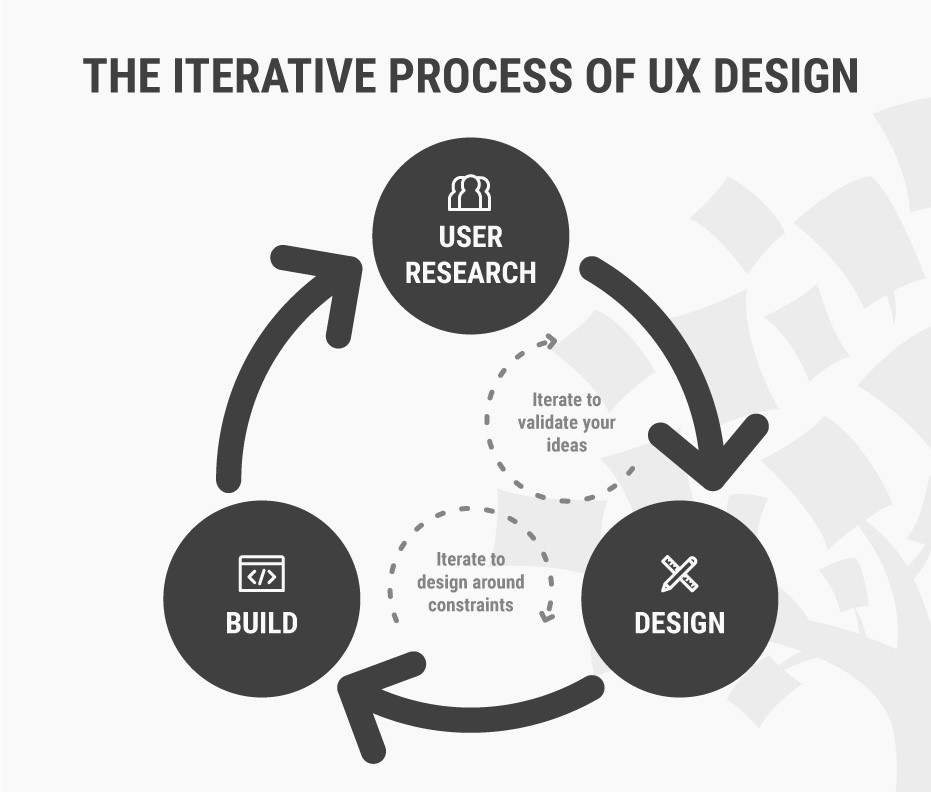
\includegraphics[width=\linewidth]{figures/ux-design}
	\caption{UX-Design.}
	\label{fig:ux-design}
\end{figure}


Ideas: \\ \\

\begin{enumerate}
	\item RQ1: Traceability

\begin{itemize}
	\item Every submission to analysis tool is time stamped.
	\item Show bugs fixed / new bugs introduced
	\item  Revert option for every submission ( this could help user to ty alternative approach of fixing a certain bug )
\end{itemize}

\item RQ2: Results

\begin{itemize}
	\item Bug List ( Column - tool icons)
	\item Bug filter
	\item Old/ New Bugs - Total Bugs
	\item Categorise ( ex. Security, Memory consumption etc)
\end{itemize}

\item RQ3: Feedback

\begin{itemize}
	\item Percent bar for each bug in bug list
	\item if user other screen, right bottom with latest bug fixed attempt been seen by percent bar
	\item popup 'Try Again' and 'Cancel'
	\item Bug removed from list, - 'decision pending' status beside bug, better animation make believe system running
	\item Long time tool result check if Short time tool reported bug fixed in after time.
\end{itemize}

\end{enumerate}